\chapter{Perifer interaktion}
\label{PeriferInteratkion}
%
\begin{itemize}
  \item Perifer interaktion - de to yderpunkter
  \item Opmærksomhed (perifer opmærksomhed)
  \item Inddrag figur fra projektforslag (side 118 i bogen eller side 6, der er den røde cirkel der ikke)
  \item Hvorfor er det interesant at designe produkter, som kan reagere på perifer interaktion? (fordele og ulemper) 
  \item Inddrag at det er relativt nyt og ukendt at have produkter, som man kan interagere med perifert 
  \item Microgestures 
  \item Socialt acceptabelt 
  \item Hvordan har perifer interaktion ændret sig? (nu er det blevet skærmbaseret)
  \item Adfærdsændringer
  \item Relateret produkter  
\end{itemize}


%
\begin{figure}[H]
	\centering
	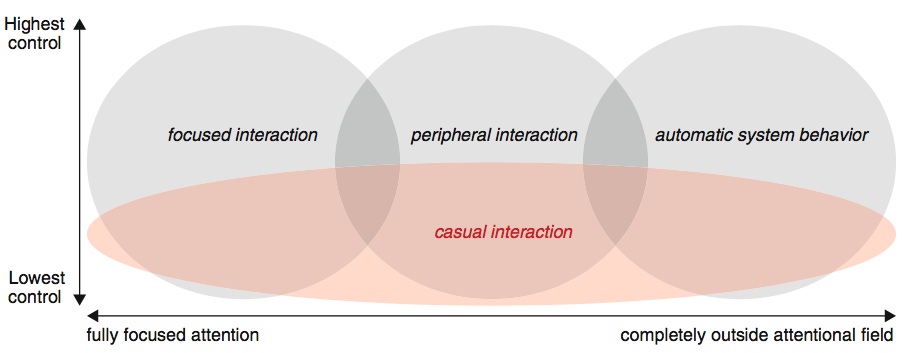
\includegraphics[resolution=300,width=\textwidth]{LevelsOfInteraction}
	\caption{ny.}
	\label{fig:LevelsOfInteraction}
\end{figure}
\noindent
%